\section{Measure Theory}
\begin{enumerate}
\item A thorough and rigorous study of probability theory \emph{requires}
measure theory. While you may have learnt probability without ever using
measure theory before (typically the case for a first course in probability),
many concepts and terminologies you have seen are in fact measure theoretic.
For example, an \emph{event} is a \emph{measurable} set, and a \emph{random
variable} is a \emph{measurable} function. For now, you may not find the need
of introducing measure theory in the study of probability. But as we shall see
very soon, there are some ``pathological'' situations that have to be handled
via measure theory.

\item As you know from your first course in probability, \emph{events} are
described as sets, so let us study/review some preliminary concepts in set
theory that will be helpful for developing measure theoretic probability
theory.
\end{enumerate}
\subsection{Set Theory Preliminaries}
\begin{enumerate}
\item Informally, a \emph{set} can be seen as a collection of distinct objects
or \emph{elements}.\footnote{Sometimes the terms ``set'' and ``collection'' are
used interchangeably. Another related term is \emph{family}, which can be
understood as a set, but repetition of elements is allowed. Often, this slight
distinction between \emph{set} and \emph{family} is not important and can be
glossed over without any issue.} While it appears to be intuitive that such
collection can be arbitrary and unrestricted, some paradoxes can actually
result if no restriction is imposed, e.g., Russell's paradox. Such issues lead
to the development of \emph{Zermelo-Fraenkel} (ZF) set theory, which imposes a
series of axioms that restrict what such ``collection'' can be.\footnote{Here we shall
not delve into the details. If you are interested, you can take a look at
\href{https://en.wikipedia.org/wiki/Zermelo%E2%80%93Fraenkel_set_theory}{its
Wikipedia page}.}

On top of the axioms in the ZF set theory, another commonly imposed axiom is
the \emph{axiom of choice}, which suggests that for any collection
\(\mathcal{A}\) of non-empty sets, there is a \emph{choice function} \(f\) such
that \(f(A)\in A\) for any \(A\in\mathcal{A}\). Intuitively, this axiom means
that it is possible to ``choose''/``pick'' an element from each set in any
fixed collection (finite or countably infinite or even uncountably infinite).

The ZF set theory together with the axiom of choice is abbreviated as
\emph{ZFC}, and we shall always work with ZFC (which is typically the case when
you encounter any mathematics involving sets).

\item \textbf{Set terminologies.} In the following, we will review
some terminologies about sets, which should be very familiar to you. Here, we
let \(\Omega\) be a nonempty \emph{universal} set (meaning that every set below
is a \emph{subset} of it).
\begin{center}
\begin{tabular}{lll}
\toprule
Name&Notation&Definition \\
\midrule
\makecell[l]{\(A\) is a subset of \(\Omega\), or \\
\(\Omega\) is a superset of \(A\)
}&
\makecell[l]{\(A\subseteq \Omega\), or \\
\(\Omega\supseteq A\)
}
&\(\omega\in A\implies \omega\in\Omega\) for any \(\omega\in A\) \\
\midrule
(Absolute) complement&\(A^c\)&\(\{\omega\in\Omega:\omega\notin A\}\) \\
Set difference&\(A\setminus B\)&\(A\cap B^c\) \\
Intersection (\(I\): index set)&\(\bigcap_{i\in I}A_i\)&\(\{\omega\in\Omega:\omega\in A_i\text{ for any \(i\in I\)}\}\) \\
Union &\(\bigcup_{i\in I}A_i\)&\(\{\omega\in\Omega:\omega\in A_i\text{ for some \(i\in I\)}\}\) \\
\midrule
Disjoint union &\(\bigsqcup_{i\in I}A_i\)&\makecell[l]{ meaning the same as \(\bigcup_{i\in I}A_i\),\\
 with the emphasis on the pairwise disjointness, \\
i.e., \(A_{i}\cap A_{j}\) for any \(i,j\in
I\) with \(i\ne j\).
}
 \\
\bottomrule
\end{tabular}
\end{center}
\begin{note}
The concept of complement depends on what the universal set is. In some
occasions, we may use the somewhat awkward notation \(A^{c_{\Omega}}\) to
stress that the universal set being considered is \(\Omega\) for this
complement.
\end{note}
\item \textbf{Basic set properties.} You should be no stranger to the following
properties of sets: (the sets below are arbitrary)
\begin{itemize}
\item \emph{Associativity of union and intersection:} \((A\cup B)\cup C=A\cup
(B\cup C)\) and \((A\cap B)\cap C=A\cap (B\cap C)\).
\item \emph{Commutativity of union and intersection:} \(A\cup B=B\cup A\) 
and \(A\cap B=B\cap A\).
\item \emph{De Morgan's laws:} \((\bigcup_{i\in I}A_i)^{c}=\bigcap_{i\in I}A_i^{c}\)
and \((\bigcap_{i\in I}A_i)^{c}=\bigcup_{i\in I}A_i^{c}\).
\end{itemize}
Make sure you are able to \emph{prove} these! (An useful way to prove a set
equality \(S=T\) is to prove (i) \(S\subseteq T\) and (ii) \(T\subseteq S\).)

\item\label{it:further-set-term} \textbf{Further set terminologies.} For the
following set theoretic terminologies, you may not have encountered them
before, so perhaps you should pay more attention here:
\begin{center}
\begin{tabular}{lll}
\toprule
Name&Notation&Definition \\
\midrule
\defn{Infimum (set)}&\(\inf_{k\ge n}A_k\)&\(\bigcap_{k\ge n}A_k\)\\
\defn{Supremum (set)}&\(\sup_{k\ge n}A_k\)&\(\bigcup_{k\ge n}A_k\) \\
\defn{Limit inferior (set)}&\(\liminf_{n\to\infty}A_n\)&\(\bigcup_{n=1}^{\infty}\bigcap_{k\ge n}A_k
=\sup_{n\ge 1}\inf_{k\ge n}A_k\)\\
\defn{Limit superior (set)}&\(\limsup_{n\to \infty}A_n\)&\(\bigcap_{n=1}^{\infty}\bigcup_{k\ge n}A_k
=\inf_{n\ge 1}\sup_{k\ge n}A_k\) \\
\defn{Limit of \(A_n\)}&\(A=\lim_{n\to \infty}A_n\) or \(A_n\to A\)&
\(\liminf_{n\to \infty}A_n=\limsup_{n\to\infty}A_n=A\) \\
\(\{A_n\}_{n\in\N}\) is \defn{increasing}&\(A_n\nearrow\)&\(A_1\subseteq A_2\subseteq\dotsb\) \\
\(\{A_n\}_{n\in\N}\) is \defn{decreasing}&\(A_n\searrow\)&\(A_1\supseteq A_2\supseteq\dotsb\) \\
\bottomrule
\end{tabular}
\end{center}
\item \textbf{Further set properties.} Here we will discuss some results about
the less familiar set terminologies from \labelcref{it:further-set-term}:
\begin{enumerate}
\item \label{it:liminfsup-interpet} \emph{(Interpreting limit inferior and limit superior)}
\begin{enumerate}
\item \(\liminf_{n\to \infty}A_n=\{\omega\in\Omega:\omega\in A_n\text{ for
\underline{a}ll \underline{b}ut \underline{f}initely \underline{m}any \(n\)}\}
=:\{\omega\in A_n\text{ abfm}\}\).
\item
\(\limsup_{n\to \infty}A_n=\{\omega\in\Omega:\omega\in A_n\text{ for infinitely many \(n\)}\}
=\{\omega\in\Omega:\omega\in A_n\text{ \underline{i}nfinitely \underline{o}ften}\}
=:\{\omega\in A_n\text{ io}\}\).
\end{enumerate}
\begin{pf}
\begin{enumerate}
\item Note that
\[
\liminf_{n\to \infty}A_n=\bigcup_{n=1}^{\infty}\bigcap_{k\ge n}A_k
=\{\omega\in\Omega:\exists n\in\N\text{ s.t. }\omega\in A_k\;\forall k\ge n\}
\]
and ``\(\exists n\in\N\text{ s.t. }\omega\in A_k\;\forall k\ge n\)'' just means
``\(\omega\in A_n\) for all but finitely many \(n\)'' in words.

\item Similar to above, and we can interpret ``\(\forall n\in\N\; \exists k\ge
n\text{ s.t. }\omega\in A_k\)'' as \(\omega\in A_n\) for infinitely many \(n\).
\end{enumerate}
\end{pf}
\item \label{it:liminfsup-relate} \emph{(Relating limit inferior and limit superior)}
\begin{enumerate}
\item \(\liminf_{n\to \infty}A_n\subseteq \liminf_{n\to \infty}A_n \).
\item \((\liminf_{n\to \infty}A_n)^{c}=\limsup_{n\to \infty}A_n^c \).
\item \((\limsup_{n\to \infty}A_n)^{c}=\liminf_{n\to \infty}A_n^c \).
\end{enumerate}
\begin{pf}
\begin{enumerate}
\item Because ``\(\omega\in A_n\) for all but finitely many \(n\)'' is just a
special case of ``\(\omega\in A_n\) for infinitely many \(n\)''.
\item Apply De Morgan's laws twice:
\[
\qty(\liminf_{n\to \infty}A_n)^{c}
=\qty(\bigcup_{n=1}^{\infty}\vc{\bigcap_{k\ge n}A_k})^{c}
\overset{\text{DM}}{=} \bigcap_{n=1}^{\infty}\vc{\qty(\bigcap_{k\ge n}A_k)^{c}}
\overset{\text{DM}}{=} \bigcap_{n=1}^{\infty}\qty(\vc{\bigcup_{k\ge n}A_k^{c}})
=\limsup_{n\to \infty}A_n^c .
\]
\item Again apply De Morgan's laws twice:
\[
\qty(\limsup_{n\to \infty}A_n)^{c}
=\qty(\bigcap_{n=1}^{\infty}\vc{\bigcup_{k\ge n}A_k})^{c}
\overset{\text{DM}}{=} \bigcup_{n=1}^{\infty}\vc{\qty(\bigcup_{k\ge n}A_k)^{c}}
\overset{\text{DM}}{=} \bigcup_{n=1}^{\infty}\qty(\vc{\bigcap_{k\ge n}A_k^{c}})
=\liminf_{n\to \infty}A_n^c .
\]
\end{enumerate}
\end{pf}
\item \label{it:lim-mono-sets} \emph{(Limits of monotone sequences of sets)}
\begin{enumerate}
\item If \(A_n\nearrow\), then \(\lim_{n\to \infty}A_n\) exists and equals \(\bigcup_{k=1}^{\infty} A_k\).
\item If \(A_n\searrow\), then \(\lim_{n\to \infty}A_n\) exists and equals \(\bigcap_{k=1}^{\infty} A_k\).
\item For any collection \(\{A_n\}\subseteq\pow{\Omega}\), \(\liminf_{n\to \infty}A_n
=\lim_{n\to \infty}(\inf_{k\ge n}A_k)\) and \(\limsup_{n\to \infty}A_n
=\lim_{n\to \infty}(\sup_{k\ge n}A_k)\). \begin{note}
This explains the rationale behind the notations ``\(\liminf_{n\to
\infty}A_n\)'' and ``\(\limsup_{n\to \infty}A_n\)''.
\end{note}
\end{enumerate}
\begin{pf}
\begin{enumerate}
\item Assuming \(A_n\nearrow\), we have \vc{\(A_k\subseteq
\bigcap_{i=k}^{\infty}A_i\)}. Hence,
\[
\limsup_{n\to \infty}A_n=\bigcap_{n=1}^{\infty}\bigcup_{k=n}^{\infty}A_k
\subseteq \boxed{\bigcup_{k=1}^{\infty}\vc{A_k}}
\vc{\subseteq} \bigcup_{n=1}^{\infty}\vc{\bigcap_{i=k}^{\infty}A_i}
=\liminf_{n\to \infty}A_n
\subseteq \limsup_{n\to \infty}A_n.
\]
This forces \(\liminf_{n\to \infty}A_n=\limsup_{n\to
\infty}A_n=\bigcup_{k=1}^{\infty}A_k\), as desired.

\item Let \(B_n=A_n^c\) for every \(n\), then \(B_n\nearrow\). Applying (i), we
get
\[
\liminf_{n\to \infty}B_n
=\limsup_{n\to \infty}B_n
=\bigcup_{k=1}^{\infty}B_k.
\]
By \labelcref{it:liminfsup-relate}, we have \(\liminf_{n\to
\infty}B_n=(\limsup_{n\to \infty}A_n)^c\) and
\(\limsup_{n\to \infty}B_n=(\liminf_{n\to \infty}A_n)^c\). It then follows that
\[
\liminf_{n\to \infty}A_n=\limsup_{n\to \infty}A_n=\qty(\bigcup_{k=1}^{\infty}B_k)^c
=\bigcap_{k=1}^{\infty}A_k^{c}.
\]
\item Note that \(\inf_{k\ge n}A_k\nearrow\) and \(\sup_{k\ge n}A_k\searrow\).
Hence,
\[
\liminf_{n\to \infty}A_n=\bigcup_{n=1}^{\infty}\bigcap_{k=n}^{\infty}A_k
=\bigcup_{n=1}^{\infty}\inf_{k\ge n}A_k
\overset{\text{(i)}}{=}\lim_{n\to \infty}\qty(\inf_{k\ge n}A_k)
\]
and
\[
\limsup_{n\to \infty}A_n=\bigcap_{n=1}^{\infty}\bigcup_{k=n}^{\infty}A_k
=\bigcap_{n=1}^{\infty}\sup_{k\ge n}A_k
\overset{\text{(ii)}}{=}\lim_{n\to \infty}\qty(\sup_{k\ge n}A_k).
\]
\end{enumerate}
\end{pf}
\end{enumerate}
\item \textbf{Equivalence relations.} Concepts related to equivalence relation
have been discussed in MATH2012; here we will go through some key points:
\begin{itemize}
\item An \emph{equivalence relation} is a relation \(\sim\) on a set \(A\) that is
(i) reflexive: \(a\sim a\), (ii) symmetric: \(a\sim b\implies b\sim a\), and
(iii) transitive: \(\text{\(a\sim b\) and \(b\sim c\)}\implies a\sim c\).
(where \(a,b,c\) are all arbitrary elements in \(A\)).
\item The \emph{equivalence class} of \(a\in A\) under an equivalence relation
\(\sim\) on \(A\) is \([a]:=\{x\in A:x\sim a\}\), i.e., the set of all elements
in \(A\) that are ``equivalent'' to \(a\) under \(\sim\).
\item Property: Two equivalence classes are either identical or disjoint, and
\([a]=[b]\) iff \(a\sim b\).
\item Property: The set of all distinct equivalence classes, \(P=\{[a]:a\in
A\}\), forms a partition of \(A\) (i.e., the classes in \(P\) are pairwise
disjoint and their union is \(A\)).
\end{itemize}
\item \textbf{Indicator functions.} You should have learnt what an indicator
function is in your first probability course. This function continues to be of
great use here, so let us review it a bit.
\begin{itemize}
\item The \emph{indicator function} of \(A\subseteq \Omega\) is given by
\[
\indic_{A}(\omega)=\begin{cases}
1&\text{if \(\omega\in A\),} \\
0&\text{otherwise.} \\
\end{cases}
\]
\item Property: \(\indic_{A}\le\indic_{B}\) (i.e.,
\(\indic_{A}(\omega)\le\indic_{B}(\omega)\) for any \(\omega\in\Omega\)) iff
\(A\subseteq B\).
\end{itemize}
Indicator function can be applied for describing \(\limsup_{n\to \infty}A_n\)
and \(\liminf_{n\to \infty}A_n\):
\[
\limsup_{n\to \infty}A_n=\qty{\omega\in\Omega:\sum_{n=1}^{\infty}\indic_{A_n}(\omega)=\infty},\quad
\liminf_{n\to \infty}A_n=\qty{\omega\in\Omega:\sum_{n=1}^{\infty}\indic_{A_{n}^{\rc{c}}}(\omega)<\infty}.
\]
This is because when \(\omega\in A_n\) infinitely often, infinitely many
\(\indic_{A_n}(\omega)\) would equal one; when \(\omega\in A_n\) for all but
finitely many \(n\), finitely many \(\indic_{A_n^{\rc{c}}}(\omega)\) would
equal one.

\item \textbf{Images and preimages.} A pair of concepts that will frequently
appear in our discussion of measure theory is \emph{image} and \emph{preimage},
which is again covered in MATH2012.

Let \(\Omega\) and \(\Omega'\) be two sets, and \(X:\Omega\to\Omega'\) be a
function.  The \emph{image} of \(A\subseteq \Omega\) under \(X\) is
\(X(A):=\{X(\omega):\omega\in A\}\), and the \emph{preimage} of \(A'\subseteq
\Omega'\) under  is \(X^{-1}(A'):=\{\omega\in\Omega:X(\omega)\in A'\}\).
\begin{center}
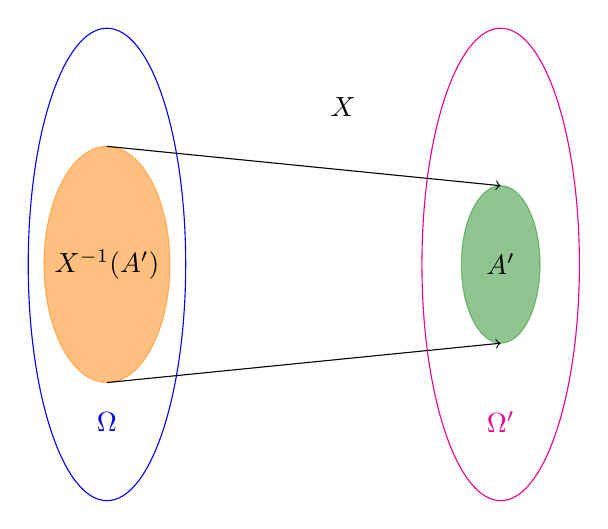
\begin{tikzpicture}
\draw[blue] (0,0) ellipse [x radius=1cm, y radius=3cm];
\draw[magenta] (5,0) ellipse [x radius=1cm, y radius=3cm];
\draw[ForestGreen, fill, opacity=0.5] (5,0) ellipse [x radius=0.5cm, y radius=1cm];
\draw[orange, fill, opacity=0.5] (0,0) ellipse [x radius=0.8cm, y radius=1.5cm];
\draw[->] (0,1.5) -- (5,1);
\draw[->] (0,-1.5) -- (5,-1);
\node[] () at (0,0) {\(X^{-1}(A')\)};
\node[] () at (5,0) {\(A'\)};
\node[] () at (3,2) {\(X\)};
\node[blue] () at (0,-2) {\(\Omega\)};
\node[magenta] () at (5,-2) {\(\Omega'\)};
\end{tikzpicture}
\end{center}
Let \(\mathcal{A}'\) be a family/set of sets in \(\Omega'\) (i.e., a
subfamily/subset of \(\mathcal{P}(\Omega')\). Then, the notation
\(X^{-1}(\mathcal{A}')\) refers to the family/set of all preimages of sets in
\(\mathcal{A}\), i.e., \(\{X^{-1}(A'):A'\in\mathcal{A}'\}\).
\item\label{it:preimg-prop} \textbf{Properties of preimages.} Let \(A',B'\)
denote any subsets of \(\Omega'\), and \(\{A_i'\}_{i\in I}\) be any
subcollection in \(\mathcal{P}(\Omega')\).
\begin{enumerate}
\item \emph{(preservation of complementation)} \(\big(X^{-1}(A')\big)^{c}=X^{-1}(A'^{c})\).
\item \emph{(preservation of union)} \(X^{-1}(\bigcup_{i\in I}A_i')=\bigcup_{i\in I}X^{-1}(A_i')\).
\item \emph{(preservation of intersection)} \(X^{-1}(\bigcap_{i\in I}A_i')=\bigcap_{i\in I}X^{-1}(A_i')\).
\item \emph{(monotonicity)} Let \(\mathcal{A}',\mathcal{B}'\subseteq
\mathcal{P}(\Omega')\). Then, \(\mathcal{A}'\subseteq \mathcal{B}'\implies
X^{-1}(\mathcal{A}')\subseteq X^{-1}(\mathcal{B}')\).
\end{enumerate}
\begin{pf}
We demonstrate the proof for (b) and (d) here and leave the rest as exercises.

\begin{enumerate}
\item[(b)]
``\(\subseteq\)'': Fix any \(\omega\in X^{-1}(\bigcup_{i\in I}A_i')\). By
definition, \(X(\omega)\in\bigcup_{i\in I}A_i'\), thus there exists some \(i\in
I\) such that \(X(\omega)\in A_i'\), or \(\omega\in X^{-1}(A_i')\). This means
\(\omega\in \bigcup_{i\in I}X^{-1}(A_i')\).

``\(\supseteq\)'': Highly similar to ``\(\subseteq\)''; just work backward.

\item[(d)] Assume \(\mathcal{A}'\subseteq \mathcal{B}'\). Now, fix any \(A\in
X^{-1}(\mathcal{A}')\). By definition, we have \(A=X^{-1}(A')\) for some
\(A'\in\mathcal{A}'\). Since \(\mathcal{A}'\subseteq \mathcal{B}'\), we also
have \(A'\in\mathcal{B}'\), meaning that
\(A\in\{X^{-1}(A'):A'\in\mathcal{B}'\}=X^{-1}(\mathcal{B}')\).
\end{enumerate}
\end{pf}
\end{enumerate}
\subsection{Non-Measurable Sets}
\begin{enumerate}
\item A critical concept in measure theory is \emph{measurable set}. Roughly
speaking, it refers to any set whose ``volume'' (or ``length'', or ``area'', or
\emph{probability} later...) can be measured. A natural and important question
is then, are there really sets that \emph{cannot} be measured? The answer is
yes, and actually the existence of \emph{non-measurable} sets leads to many
interesting and fruitful developments in measure theory.

\item\label{it:meas-intuitive} Before discussing non-measurable sets, let us
first consider what is meant by ``measure'' intuitively\footnote{We will define
\emph{measure} more formally later.}. First, we can view a measure as a
function \(\lambda\) that assigns a value (``volume'') to a set. For
simplicity, let us first focus on the case where the universal set is
\(\Omega=\R\).

A ``reasonable measure'' \(\lambda:\mathcal{F}\to [0,\infty]\)\footnote{The
domain \(\mathcal{F}\) is a family of sets in \(\Omega=\R\). We choose the
codomain as \([0,\infty]\) since it makes sense for a ``volume'' to be always
nonnegative, and we sometimes want to assign ``infinite volume''.} should
satisfy the following:
\begin{enumerate}[label={(\arabic*)}]
\item \emph{(assigning to an interval its length)} \(\lambda((a,b])=b-a\) for
any \(a,b\in\R\) with \(a\le b\).  Here, \(a,b]\) can be replaced by
\((a,b)\), \([a,b\), or \([a,b]\).
\item \emph{(invariant under translation, rotations, and reflections)}
\(\lambda\) assigns the same value to \emph{congruent} sets (i.e., one can be
obtained from another using just translations, rotations, and reflections).
\item \emph{(\(\sigma\)-additivity)} Given any pairwise disjoint collection
\(\{A_i\}_{i\in\N}\subseteq \pow{\R}\), we have
\(\lambda(\bigsqcup_{i=1}^{\infty}A_i)=\sum_{i=1}^{\infty}\lambda(A_i)\).

\begin{note}
While \emph{additivity} appears to be a more natural requirement (obtained
by changing \(\N\to\{1,\dotsc,n\}\) and \(\infty\to n\) above), the
``\(\sigma\)-'' turns out to be necessary to avoid running into technical
issues. See \Cref{thm:banach-tarski} for more discussions on this.
\end{note}
\end{enumerate}
Based on these requirements, we can deduce:
\begin{itemize}
\item \(\lambda(\varnothing)=0\) (as
\(\lambda(\varnothing)=\lambda((a,a])=a-a=0\)).
\item \emph{(additivity)} For any \(\{A_i\}_{i=1}^{n}\subseteq\pow{\R}\), we have
\(\lambda(\bigsqcup_{i=1}^{n}A_i)=\sum_{i=1}^{n}\lambda(A_i)\).
(This is because \(\lambda(\bigsqcup_{i=1}^{n}A_i)=\lambda(\bigsqcup_{i=1}^{n}A_i\sqcup\varnothing\sqcup\varnothing\sqcup\dotsb)
\overset{\text{\(\sigma\)-add.}}{=}\sum_{i=1}^{n}\lambda(A_i)+\sum_{i=n+1}^{\infty}0=\sum_{i=1}^{n}\lambda(A_i)\).)
\item \emph{(monotonicity)} For any \(A\subseteq B\), we have
\(\lambda(B)=\lambda(B\sqcup(B\setminus A))=\lambda(A)
+\underbrace{\lambda(B\setminus A)}_{\ge 0}\ge \lambda(A)\).
\end{itemize}
\item Now we are ready to start discussing non-measurable sets. The idea is
that, if every set was measurable and there were not non-measurable sets, then
we could simply set \(\mathcal{F}\) as \(\pow{\R}\), allowing every subset of
\(\R\) to be measured by \(\lambda\) (being ``measurable'' in this sense). Now,
the issue is that, setting \(\mathcal{F}=\pow{\R}\) would actually lead to a
contradiction \warn{} as suggested by the following theorem:

\begin{theorem}[Vitali's theorem]
\label{thm:vitali}
There is \rc{no} \(\lambda\) defined on \(\pow{\R}\) satisfying (a)-(c) in
\labelcref{it:meas-intuitive}.
\end{theorem}
\begin{pf}
The proof is by explicitly constructing a set \(V\) (known as \defn{Vitali
set}) living in \(\pow{\R}\) such that for every \(\lambda\) on \(\pow{\R}\)
satisfying (a)-(c), any choice of value for \(\lambda(V)\) would lead to a
contradiction.

\textbf{Defining equivalence relation.} We start with the interval \([0,1]\)
and define an equivalence relation \(\sim\) on \([0,1]\) by \(x\sim y\) if
\(x-y\in \Q\), or in words, two values in \([0,1]\) are ``equivalent'' (under
\(\sim\)) if they have a rational difference. (Check \(\sim\) is indeed an
equivalence relation!)

\textbf{Constructing Vitali set \(V\).} Then, the \emph{Vitali set} \(V\) is
constructed by picking exactly one element from each distinct equivalence class
under \(\sim\), and collecting them together (possible under the axiom of
choice!).  Symbolically, we can write:
\[
V=\{v\in[0,1]:\forall x\in [0,1]\; \exists! v\in [x]\}.
\]
\begin{note}
Although the condition ``\(\forall x\in [0,1]\; \exists! v\in [x]\)'' does not
only consider distinct classes (it involves all possible equivalence classes
indeed), it does not matter because for identical equivalence classes, the
same unique element \(v\) picked would apply.
\end{note}
\begin{center}
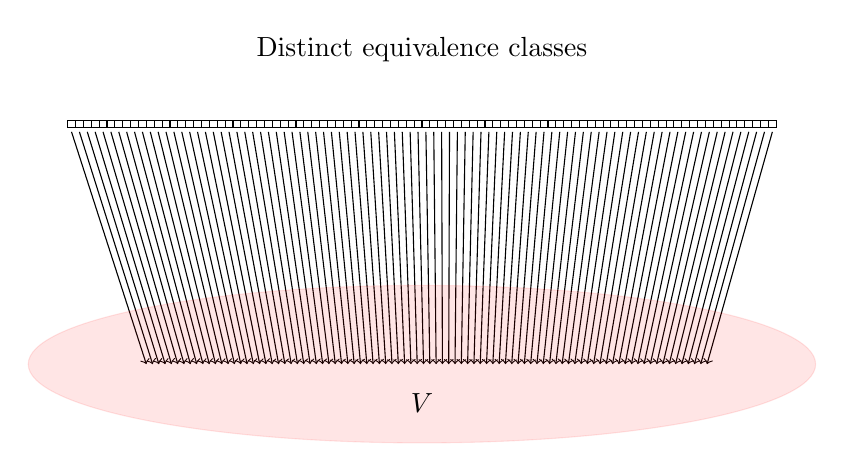
\begin{tikzpicture}
\foreach \x in {0,0.1,...,9} {
\draw[] (\x, 0) rectangle (\x+0.1, 0.1);
\draw[->] (\x+0.05, -0.05) -- (\fpeval{1+0.8*\x},-3);
}
\draw[red, fill, opacity=0.1] (4.5,-3) ellipse [x radius=5cm, y radius=1cm];
\node[] () at (4.5,-3.5) {\(V\)};
\node[] () at (4.5,1) {Distinct equivalence classes};
\end{tikzpicture}
\end{center}

\textbf{Shifting Vitali set \(V\) by rationals.}
Next, we enumerate \(\Q\cap[-1,1]\) in a similar fashion as the \emph{Cantor's
diagonal argument} (used for proving the well-known result that \(\Q\) is
countable) with repeated values or values lying outside \([-1,1]\) being
skipped, to form an infinite sequence \(\{q_k\}_{k\in\N}\) of \emph{distinct}
rational numbers in \([-1,1]\).

The rational numbers in \(\{q_k\}\) are then used to ``shift'' the Vitali set
\(V\) to yield \(V_k:=V+q_k:=\{v+q_k:v\in V\}\) for every \(k\in\N\).

\textbf{Proving two auxiliary claims.}

\textbf{Claim:} \([0,1]\subseteq \bigcup_{k=1}^{\infty}V_k\subseteq [-1,2]\).

\begin{pf}
By construction, \(V_k\subseteq [-1,2]\) for every \(k\in\N\), thus
\(\bigcup_{k=1}^{\infty}V_k\subseteq [-1,2]\). Next, fix any \(x\in [0,1]\). By
construction of \(V\), we have \(x\in [v]\) for some \(v\in V\), which means
that for some \(k\in\N\), \(x-v=q_k\) or \(x=v+q_k\in V_k\). This shows that
\([0,1]\subseteq \bigcup_{k=1}^{\infty}V_k\).
\end{pf}

\textbf{Claim:} \(V_k\)'s are pairwise disjoint.

\begin{pf}
Suppose not, then there is \(x\in V_k\cap V_j\) for some \(k\ne j\). Then, we
can write \(x=v_k+q_k\) and \(x=v_j+q_j\) for some \(v_k,v_j\in V\) and
\emph{distinct} \(q_k,q_j\in \Q\cap[-1,1]\). This implies that \(v_k=x-q_k\ne
x-q_j=v_j\). However, we have \(v_k-x=-q_k\in\Q\) and \(v_j-x=-q_j\in\Q\), thus
\(v_k\sim x\) and \(x\sim v_j\), which implies \(v_k\sim v_j\) by transitivity
(i.e., \(v_k\) and \(v_j\) are in the same equivalence class).  This means
\(V\) contains two \emph{distinct} elements in the \emph{same} equivalence
class, contradiction!
\end{pf}

\textbf{Showing the contradiction.}
With the two claims established, we can write \([0,1]\subseteq
\bigsqcup_{k=1}^{\infty}V_k\subseteq [-1,2]\). Then, by monotonicity of \(\lambda\), we have
\[
1=\lambda([0,1])\le\lambda\qty(\bigsqcup_{k=1}^{\infty}V_k)\le\lambda([-1,2])=3.
\]
Applying \(\sigma\)-additivity on \(\lambda(\bigsqcup_{k=1}^{\infty}V_k)\) gives
\(1\le\sum_{k=1}^{\infty}\lambda(V_k)\le 3\). Note that
\(\lambda(V_k)=\lambda(V)\) by the invariance under translation, so
\(\sum_{k=1}^{\infty}\lambda(V_k)=\sum_{k=1}^{\infty}\lambda(V)\). But then
this sum is either \(0\) (when \(\lambda(V)=0\)) or \(\infty\) (when
\(\lambda(V)>0\)). Neither is between \(1\) and \(3\), contradiction.
\end{pf}

The Vitali set \(V\) in the proof is an example of \emph{non-measurable} set.
Assigning a ``volume'' to \(V\) would break the mathematics. This suggests that
the power set \(\pow{\R}\) is ``too large'' and contains some ``pathological''
sets like the Vitali set. This calls for the need to define \(\lambda\) on only
a selected collection of sets, which can be constructed using the concepts to
be introduced in \Cref{subsect:set-system}.

\item But before proceeding to
\Cref{subsect:set-system}, let us explain a little bit more about the rationale
behind using \(\sigma\)-additivity rather than additivity as a requirement for
the ``reasonable measure'' \(\lambda\), through the following theorem:

\begin{theorem}[Banach-Tarski paradox]
\label{thm:banach-tarski}
Let \(d\ge 3\) be an integer, and \(A,B\subseteq \R^d\) be any bounded sets
with nonempty interior. Then, for some \(k\in\N\), there exist pairwise
disjoint collections \(\{A_i\}_{i=1}^{k}\) and \(\{B_i\}_{i=1}^{k}\) such that
\(A=\bigsqcup_{i=1}^{k}A_i\) and \(B=\bigsqcup_{i=1}^{k}B_i\) where \(A_i\) and
\(B_i\) are congruent for every \(i=1,\dotsc,k\).
\end{theorem}
\begin{pf}
It is quite technical and hence omitted.
\end{pf}

The paradoxical feature of \Cref{thm:banach-tarski} is that while there is no
limitation on how the sizes/``volumes'' of \(A\) and \(B\) can differ, e.g.,
\(A\) can be a very small ``pea \gc{\(\bullet\)}'' and \(B\) can be the very
large ``sun \faIcon{sun}'', each of them can always be decomposed into finitely
many pieces where every pair of pieces is \emph{congruent} (``same in
size'')\warn{}.  Informally, we may say that \textit{``a pea \gc{\(\bullet\)}
can be chopped up and reassembled into the sun \faIcon{sun}''}. What went wrong
here?

The main issue is again related to non-measurable sets. We claim that at least
one set in the collections \(\{A_i\}_{i=1}^{k}\) and \(\{B_i\}_{i=1}^{k}\) is
non-measurable. If not, additivity would imply that
\(\lambda(A)=\lambda(\bigsqcup_{i=1}^{k}A_i)=\sum_{i=1}^{k}\lambda(A_i)
\overset{\text{invariance}}{=}\sum_{i=1}^{k}\lambda(B_i)=\lambda(\bigsqcup_{i=1}^{k}B_i)=\lambda(B)\).
But we can select \(A\) and \(B\) that get different assigned values by
\(\lambda\). Contradiction.
\end{enumerate}
\subsection{Systems of Sets}
\label{subsect:set-system}
\begin{enumerate}
\item \emph{Systems of sets} are utilized for constructing families of
``selected'' sets on which a ``reasonable measure'' \(\lambda\) can be defined
consistently without having any issue. There are multiple systems of sets here,
but they all share a common theme, which is about constructing a family of
sets that is \emph{closed} under certain set operations, i.e., performing
these operations on sets in \(\mathcal{F}\) would not yield something outside
\(\mathcal{F}\) --- being ``stable'' in some sense.  Intuitively, we are
interested in this kind of properties because they can make the families
of sets ``rich enough'', in the sense that the families contain ``sufficiently
many well-behaved sets''.

The systems of sets to be discussed here are: (i) semiring, (ii) ring, (iii)
algebra, and (iv) \ystar{} \(\sigma\)-algebra (important concept for
probability theory!).

\item \textbf{Definitions.}
\begin{itemize}
\item A family \(\mathcal{A}\subseteq \pow{\Omega}\) is a \defn{semiring} on
\(\Omega\) if
\begin{enumerate}[label={(\arabic*)}]
\item \(\varnothing\in\mathcal{A}\).
\item \emph{(``stable'' under set differences)}
\(A,B\in\mathcal{A}\implies A\setminus B=\bigsqcup_{i=1}^{n}A_i\) for
some pairwise disjoint \(A_1,\dotsc,A_n\in\mathcal{A}\), where \(n\in\N\).
\item \emph{(closed under intersections)} \(A,B\in\mathcal{A}\implies A\cap B\in\mathcal{A}\).
\end{enumerate}
\begin{note}
The ``stability'' under set differences suggests that, while taking set
differences may yield something outside \(\mathcal{A}\), we can still express
the result as a disjoint union of finitely many sets in \(\mathcal{A}\) (so
still ``stable'' to a certain degree).
\end{note}
\item A family \(\mathcal{A}\subseteq \pow{\Omega}\) is a \defn{ring} on \(\Omega\) if
\begin{enumerate}[label={(\arabic*)}]
\item \(\varnothing\in\mathcal{A}\).
\item \emph{(closed under set differences)}
\(A,B\in\mathcal{A}\implies A\setminus B\in\mathcal{A}\).
\item \emph{(closed under unions)} \(A,B\in\mathcal{A}\implies A\cup B\in\mathcal{A}\).
\end{enumerate}
\item A family \(\mathcal{A}\subseteq \pow{\Omega}\) is an \defn{algebra} (or
\defn{field}) on \(\Omega\) if
\begin{enumerate}[label={(\arabic*)}]
\item \(\varnothing\in\mathcal{A}\).
\item \emph{(closed under complementations)} \(A\in\mathcal{A}\implies A^c=\Omega\setminus A\in\mathcal{A}\).
\item \emph{(closed under unions)}
\(A,B\in\mathcal{A}\implies A\cup B\in\mathcal{A}\).
\end{enumerate}
\item \ystar{} A family \(\mathcal{A}\subseteq \pow{\Omega}\) is a
\defn{\(\sigma\)-algebra} (or \defn{\(\sigma\)-field}) on \(\Omega\) if
\begin{enumerate}[label={(\arabic*)}]
\item \(\varnothing\in\mathcal{A}\).
\item \emph{(closed under complementations)} \(A\in\mathcal{A}\implies A^c=\Omega\setminus A\in\mathcal{A}\).
\item \emph{(closed under countable unions)}
\(A_1,A_2,\dotsc\in\mathcal{A}\implies \bigcup_{i=1}^{\infty}A_i\in\mathcal{A}\).
\end{enumerate}
\begin{note}
A \(\sigma\)-algebra is actually also closed under countable
\emph{intersections}. To show this, we can use De Morgan law, and the
closedness under countable unions and complementations.
\[
A_1,A_2,\dotsc\in\mathcal{A}
\implies \bigcap_{i=1}^{\infty}A_i\overset{\text{DM}}{=}
\qty(\bigcup_{i=1}^{\infty}A_i^{c})^{c}
\in\mathcal{A}.
\]
\end{note}
\end{itemize}
\item \textbf{Relationships between systems of sets.} It turns out that these
four systems are imposing stronger requirements in the order of introduction,
resulting in this chain of relationships:
\(\text{\(\sigma\)-algebra}\subsetneq\text{algebra}\subsetneq\text{ring}\subsetneq\text{semiring}\),
or in words, every \(\sigma\)-algebra is an algebra; every algebra is a ring;
etc., with the inclusion being strict, i.e., some algebra is not
\(\sigma\)-algebra; some ring is not algebra; etc.

\begin{proposition}[Relationships between systems of sets]
\label{prp:set-systems-relate}
\hfill
\begin{enumerate}
\item \(\text{\(\sigma\)-algebra}\subsetneq\text{algebra}\subsetneq\text{ring}\subsetneq\text{semiring}\).
\item An algebra on a \emph{finite} set \(\Omega\) is a \(\sigma\)-algebra.
\item A semiring that is also closed under unions is a ring.
\end{enumerate}
\end{proposition}
\begin{pf}
\begin{enumerate}
\item 
\begin{itemize}
\item \underline{\(\text{\(\sigma\)-algebra}\subsetneq \text{algebra}\)} \\
\textbf{Inclusion:} Fix any \(\sigma\)-algebra \(\mathcal{A}\) on \(\Omega\),
and any \(A,B\in\mathcal{A}\). Let \(A_1=A\), \(A_2=B\), and
\(A_3=A_4=\dotsb=\varnothing\). Applying closedness under countable unions, we get
\(A\cup B=\bigcup_{i=1}^{\infty}A_i\in\mathcal{A}\). This means \(\mathcal{A}\)
is closed under unions, thus is an algebra.

\textbf{Strictness:} Take \(\Omega=(0,1]\) and
\(\mathcal{A}=\{\bigsqcup_{i=1}^{n}(a_i,b_i]: 0\le a_i\le b_i\le 1, n\in\N\}\)
(or in words, the family of all possible finite disjoint unions of intervals of
the form \((a,b]\) (i.e., left-open and right-closed intervals) lying in
\(\Omega=(0,1]\)).

It can be directly checked that \(\mathcal{A}\) is an algebra.
\begin{center}
\begin{tikzpicture}
\draw[-Latex] (0,0) -- (10,0);
\node[blue] () at (2,0) {(};
\node[blue] () at (8,0) {]};
\node[blue] () at (5,0.5) {\(\Omega\)};
\node[magenta] () at (4,0) {(};
\node[magenta] () at (5,0) {]};
\node[] () at (4,-0.5) {\(a_1\)};
\node[] () at (5,-0.5) {\(b_1\)};
\node[magenta] () at (5.5,0) {(};
\node[magenta] () at (7.5,0) {]};
\node[] () at (5.5,-0.5) {\(a_2\)};
\node[] () at (7.5,-0.5) {\(b_2\)};
\draw[magenta] (4.5,-0.2) -- (6,-1);
\draw[magenta] (6.5,-0.2) -- (6,-1);
\node[] () at (6,-1.3) {\((a_1,b_1]\sqcup(a_2,b_2]\)};
\draw[line width=0.2cm, magenta, opacity=0.2] (4,0) -- (5,0);
\draw[line width=0.2cm, magenta, opacity=0.2] (5.5,0) -- (7.5,0);
\end{tikzpicture}
\begin{tikzpicture}
\draw[-Latex] (0,0) -- (10,0);
\node[blue] () at (2,0) {(};
\node[blue] () at (8,0) {]};
\node[blue] () at (5,0.5) {\(\Omega\)};
\node[ForestGreen] () at (4,0) {]};
\node[ForestGreen] () at (5,0) {(};
\node[ForestGreen] () at (5.5,0) {]};
\node[ForestGreen] () at (7.5,0) {(};
\draw[ForestGreen] (3,-0.2) -- (6,-1);
\draw[ForestGreen] (5.25,-0.2) -- (6,-1);
\draw[ForestGreen] (7.75,-0.2) -- (6,-1);
\node[] () at (6,-1.3) {\(\big((a_1,b_1]\sqcup(a_2,b_2]\big)^{c}\)};
\draw[line width=0.2cm, ForestGreen, opacity=0.2] (2,0) -- (4,0);
\draw[line width=0.2cm, ForestGreen, opacity=0.2] (5,0) -- (5.5,0);
\draw[line width=0.2cm, ForestGreen, opacity=0.2] (7.5,0) -- (8,0);
\end{tikzpicture}
\end{center}
However, \(\mathcal{A}\) is not a \(\sigma\)-algebra because we have
\((0,1)=\bigcup_{n=1}^{\infty}(0,1-1/n]\) with \((0,1-1/n]\in\mathcal{A}\) for
every \(n\), but \((0,1)\notin \mathcal{A}\) as finite disjoint union of
left-open and right-closed intervals must still be left-open and right-closed.
\item \underline{\(\text{algebra}\subsetneq\text{ring}\)} \\
\textbf{Inclusion:} Fix any algebra \(\mathcal{A}\) on \(\Omega\), and any
\(A,B\in\mathcal{A}\).  Applying closedness under complementations and unions,
we have \(A\setminus B=A\cap B^c\overset{\text{DM}}{=}(A^c\cup B)^c\in\mathcal{A}\).
This shows \(\mathcal{A}\) is closed under set differences, and hence is a
ring.

\textbf{Strictness:} Take \(\Omega=\{1\}\) and \(\mathcal{A}=\{\varnothing\}\).
It is not hard to see that \(\mathcal{A}\) is a ring, but \(\mathcal{A}\) is
not an algebra since \(\varnothing^c=\Omega=\{1\}\notin \mathcal{A}\).

\item \underline{\(\text{ring}\subsetneq\text{semiring}\)} \\
\textbf{Inclusion:} Fix any ring \(\mathcal{A}\) on \(\Omega\), and any \(A,B\in\mathcal{A}\).
Applying closedness under set differences, we get
\(A\cap \vc{B}\overset{\text{DM}}{=}A\cap\vc{(A\cap B^c)^c}
=A\setminus (A\setminus B)\in \mathcal{A}\), and also
\(A\setminus B=\underbrace{(A\setminus B)}_{\in\mathcal{A}}\sqcup\underbrace{\varnothing}_{\in \mathcal{A}}\).

\textbf{Strictness:} Take \(\Omega=\{1,2\}\) and \(\mathcal{A}=\{\varnothing,\{1\},\{2\}\}\).
It is straightforward to check that \(\mathcal{A}\) is a semiring, but
\(\mathcal{A}\) is not a ring as \(\{1\}\cup\{2\}=\{1,2\}\notin\mathcal{A}\).
\end{itemize}
\item Because every countably infinite union of sets in \(\mathcal{A}\) can
always be expressed as a finite union of sets in \(\mathcal{A}\) in such case,
by removing redundancies.
\item Assuming a semiring \(\mathcal{A}\) is closed under unions, by
induction we have \(A_1,\dotsc,A_n\in\mathcal{A}\implies
\bigcup_{i=1}^{n}A_i\in\mathcal{A}\) for any \(n\in\N\). Therefore, we have
\(A,B\in\mathcal{A}\implies A\setminus B=\bigsqcup_{i=1}^{n}A_i\in\mathcal{A}\),
meaning that \(\mathcal{A}\) is closed under set differences, hence is a ring.
\end{enumerate}
\end{pf}
\item Due to the importance of \(\sigma\)-algebra in probability theory, let us
try to understand it better through some examples.
\begin{enumerate}[label={(\arabic*)}]
\item The \defn{trivial \(\sigma\)-algebra} on \(\Omega\) is
\(\mathcal{F}=\{\varnothing,\Omega\}\).
\begin{note}
It is the \emph{smallest} \(\sigma\)-algebra on \(\Omega\), i.e., every
\(\sigma\)-algebra on \(\Omega\) is a superset of the trivial
\(\sigma\)-algebra.  This is because containing \(\varnothing\) and being
closed under complementations would force a \(\sigma\)-algebra to at least
contain \(\varnothing\) and \(\Omega\).
\end{note}

\item The power set \(\mathcal{F}=\mathcal{P}(\Omega)\) is a \(\sigma\)-algebra
on \(\Omega\). \begin{note}
It is the \emph{largest} \(\sigma\)-algebra on \(\Omega\), i.e., every
\(\sigma\)-algebra on \(\Omega\) is a subset of \(\mathcal{P}(\Omega)\) (which
follows from definition).
\end{note}

\item \textbf{Constructing a \(\sigma\)-algebra from one
set.} Start with a set \(A\subseteq \Omega\). Then consider the following two sets that partition \(\Omega\):
\[
A\qquad A^c
\]
By putting zero/one/two of them into an union, we can get 4 combinations:
\begin{itemize}
\item \emph{zero:} \(\varnothing\)
\item \emph{one:} \(A\), \(A^c\)
\item \emph{two:} \(A\cup A^c=\Omega\)
\end{itemize}
These four sets form a \(\sigma\)-algebra: \(\{\varnothing, A, A^c, \Omega\}\).
\item \textbf{Constructing a \(\sigma\)-algebra from two sets.} Here we start
with two sets \(A,B\subseteq \Omega\). Then consider the following \(2^2=4\)
sets that partition \(\Omega\): \(A\cap B\), \(A^c\cap B\), \(A\cap B^c\), and
\(A^c\cap B^c\).
\begin{center}
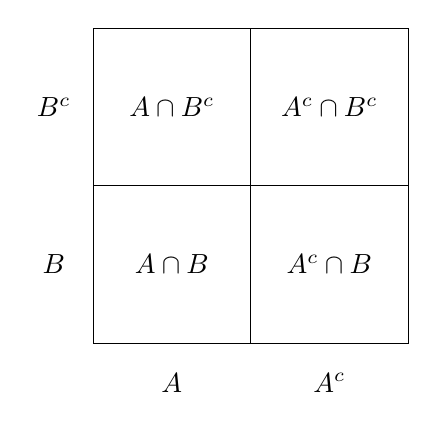
\begin{tikzpicture}
\draw[] (0,0) rectangle (2,2);
\draw[] (0,4) rectangle (2,2);
\draw[] (4,0) rectangle (2,2);
\draw[] (2,2) rectangle (4,4);
\node[] () at (1,-0.5) {\(A\)};
\node[] () at (3,-0.5) {\(A^c\)};
\node[] () at (-0.5,1) {\(B\)};
\node[] () at (-0.5,3) {\(B^{c}\)};
\node[] () at (1,1) {\(A\cap B\)};
\node[] () at (3,1) {\(A^c\cap B\)};
\node[] () at (1,3) {\(A\cap B^c\)};
\node[] () at (3,3) {\(A^c\cap B^c\)};
\end{tikzpicture}
\end{center}
By putting zero/one/two/three/four of them into an union, we can get \(\binom{4}{0}+\binom{4}{1}+\binom{4}{2}+\binom{4}{3}+\binom{4}{4}=(1+1)^4=16\) combinations:
\begin{itemize}
\item \emph{zero:} \(\varnothing\)
\item \emph{one:} \(A\cap B\), \(A^c\cap B\), \(A\cap B^c\), \(A^c\cap B^c\)
\item \emph{two:}
\begin{itemize}
\item \(B=(A\cap B)\cup(A^c\cap B)\)
\item \(A=(A\cap B)\cup(A\cap B^c)\)
\item \((A\cap B)\cup (A^c\cap B^c)\)
\item \((A^c\cap B)\cup(A\cap B^c)\)
\item \(A^c=(A^c\cap B)\cup(A^c\cap B^c)\)
\item \(B^c=(A\cap B^c)\cup(A^c\cap B^c)\)
\end{itemize}
\item \emph{three:} (just complement of each of the four sets in the partition indeed)
\begin{itemize}
\item \(A^c\cup B^c=(A\cap B)^c\)
\item \(A\cup B^c=(A^c\cap B)^c\)
\item \(A^c\cup B=(A\cap B^c)^c\)
\item \(A\cup B=(A^c\cap B^c)^c\)
\end{itemize}
\item \emph{four:} \(\Omega\)
\end{itemize}
These 16 sets form a \(\sigma\)-algebra.

\begin{note}
In general, constructing a \(\sigma\)-algebra from \(n\)
sets would yield \(2^{2^n}\) (\(\neq 4^n=2^{2n}\)) sets. This
number grows \emph{very} quickly as \(n\) rises; for
instance, constructing from \(4\) sets would already yield
\(\fpeval{2^{2^4}}\) sets! This tells us that it is almost impossible to ``visualize'' a \(\sigma\)-algebra in general (unfortunately!).
\end{note}
\item The \defn{countable-cocountable \(\sigma\)-algebra} on \(\Omega\) is
\(\mathcal{F}=\{A\subseteq \Omega:\text{\(A\) is countable or \(A^c\) is
countable}\}\). Let us prove that it is indeed a \(\sigma\)-algebra.

\begin{pf}
Since \(\varnothing\) is countable, we have \(\varnothing\in\mathcal{F}\).

Now fix any \(A\in\mathcal{F}\).
\begin{itemize}
\item \emph{Case 1: \(A\) is countable.}
Then, \((A^c)^c=A\) is countable.
\item \emph{Case 2: \(A\) is uncountable.}
Then, \(A^c\) has to be countable (or else \(A\) would not be in \(\mathcal{F}\)!).
\end{itemize}
Hence, we have \(A^c\) is countable or \((A^c)^c\) is countable, meaning that \(A^c\in\mathcal{F}\).

Next, fix any \(A_1,A_2,\dotsc\in\mathcal{F}\).
\begin{itemize}
\item \emph{Case 1: All \(A_i\)'s are countable.} Then, applying the Cantor's
diagonal argument (e.g., see \href{https://math.stackexchange.com/a/603499}{this link}), we can deduce that
\(\bigcup_{i=1}^{n}A_i\) is also countable, hence
\(\bigcup_{i=1}^{\infty}A_i\in\mathcal{F}\).
\item \emph{Case 2: \(A_k\) is uncountable for some \(k\in\N\).} Then \(A_k^c\)
has to be countable. Since
\((\bigcup_{i=1}^{\infty}A_i)^c=\bigcap_{i=1}^{\infty}A_i^c\subseteq A_k^{c}\),
the complement \((\bigcup_{i=1}^{\infty}A_i)^c\) is forced to be countable,
thus \(\bigcup_{i=1}^{\infty}A_i\in\mathcal{F}\).
\end{itemize}
\end{pf}
\item Let \(\mathcal{F}\) be an \(\sigma\)-algebra on
\(\Omega\) and \(\Omega'\subseteq \Omega\). The \defn{trace
\(\sigma\)-algebra} of \(\Omega'\) in \(\mathcal{F}\) is
\(\mathcal{F}'=\mathcal{F}|_{\Omega'}:=\{A\cap \Omega':A\in\mathcal{F}\}\).
Let us verify that the trace \(\sigma\)-algebra is indeed an \(\sigma\)-algebra
below.

\begin{pf}
Firstly, we have
\(\varnothing=\varnothing\cap\Omega'\in\mathcal{F}'\).

Next, fix any \(A'\in\mathcal{F}'\). By definition, we can write \(A'=A\cap\Omega'\) for some \(A\in\mathcal{F}\). Then, emphasizing universal sets in the complement notations, we have
\[
(A')^{c_{\Omega'}}
=(A\cap\Omega')^{c_{\Omega'}}
\overset{\text{DM}}{=}
=A^{c_{\Omega'}}\cup \Omega'^{c_{\Omega'}}
=A^{c_{\Omega'}}
=\underbrace{A^{c_{\mgc{\Omega}}}}_{\in\mathcal{F}}\cap\Omega'
\in\mathcal{F}'.
\]
Finally, fix any \(A_1',A_2',\dotsc\in\mathcal{F}\). Then, for any \(i\in\N\), we have
\(A_i'=A_i\cap\Omega'\) for some \(A_i\in\mathcal{F}\).
Hence,
\[
\bigcup_{i=1}^{\infty}A_i'
=\bigcup_{i=1}^{\infty}(A_i\cap\Omega')
\overset{\text{distributive}}{=}
\underbrace{\qty(\bigcup_{i=1}^{\infty}A_i)}_{\in\mathcal{F}}\cap\Omega'
\in\mathcal{F}'.
\]
\end{pf}
\item Let \(X:\Omega\to\Omega'\) be a function, and
\(\mathcal{F}'\) be a \(\sigma\)-algebra on \(\Omega'\).
Then, the \defn{\(\sigma\)-algebra generated by \(X\)} or \defn{preimage \(\sigma\)-algebra} is
\[
\mathcal{F}=\sigma(X):=X^{-1}(\mathcal{F}')
=\{X^{-1}(A'):A'\in\mathcal{F}'\},
\]
which is indeed a \(\sigma\)-algebra.

\begin{pf}
First, we have \(\varnothing=X^{-1}(\underbrace{\varnothing}_{\in\mathcal{F}'})\in\mathcal{F}\).

Now fix any \(A\in\mathcal{F}\). Then \(A=X^{-1}(A')\) for some
\(A'\in\mathcal{F}'\). Hence,
\[
A^{c}=(X^{-1}(A'))^{c}\overset{\text{preserv.\ comp.}}{=}
X^{-1}(\underbrace{(A')^{c}}_{\in\mathcal{F}'})
\in\mathcal{F}.
\]
Next, fix any \(A_1,A_2,\dotsc\in\mathcal{F}\). Then for any \(i\in\N\),
\(A_i=X^{-1}(A_i')\) for some \(A_i'\in\mathcal{F}'\). Thus,
\[
\bigcup_{i=1}^{\infty}A_i
=\bigcup_{i=1}^{\infty}X^{-1}(A_i')
\overset{\text{preserv.\ union}}{=}
X^{-1}\bigg(\underbrace{\bigcup_{i=1}^{\infty}A_i'}_{\in\mathcal{F}'}\bigg)
\in\mathcal{F}.
\]
\end{pf}
\item The last example is about an important concept in the theory of
stochastic process, called \emph{filtration}. A \defn{filtration} is an
increasing sequence \(\mathcal{F}_1\subseteq \mathcal{F}_2\subseteq \dotsb\) of
\(\sigma\)-algebras on \(\Omega\). It is useful for modelling \emph{information}
accrued over time.

\begin{note}
Here we will use some of your prior probability knowledge.
\end{note}
Suppose we model an experiment of tossing a coin
(countably) infinitely many times by setting the sample space as
\[
\Omega=\{0,1\}^{\infty}:=\{\vect{\omega}=(\omega_1,\omega_2,\dotsc):\omega_1,\omega_2,\dotsc\in\{0,1\}\}
\]
with ``\(0\)'' and ``\(1\)'' being labels for ``tails' and ``heads''
respectively, say.

For each \(n\in\N\), let
\[\mathcal{F}_n=\big\{\{\vect{\omega}\in\Omega:(\omega_1,\dotsc,\omega_n)\in
A\}: A\subseteq \{0,1\}^{n}\big\},
\]
the set of all events whose \emph{occurrence can be decided after the
first \(n\) tosses}. For example, the event ``2nd toss is heads'',
\(\{\vect{\omega}\in\Omega:\text{2nd toss is heads}\}
=\{\vect{\omega}\in\Omega:\omega_2=1\}\), belongs to \(\mathcal{F}_2\) but not
\(\mathcal{F}_1\), because the \emph{information} about 2nd toss is only known
to us after the first 2 tosses!

Here, we can see that \(\mathcal{F}_n\) is somewhat like a set of
``information'' available to us after the first \(n\) tosses. The property that
\(\mathcal{F}_{1}\subseteq \mathcal{F}_2\subseteq\dotsb \) corresponds to the
fact that ``more information accrues over time''.  This increasing sequence is
indeed a filtration as well:

\textbf{Claim:} \(\mathcal{F}_n\) is a \(\sigma\)-algebra on \(\Omega\) for each \(n\in\N\).

\begin{pf}
Fix any \(n\in\N\).

First, by taking \(A=\varnothing\), we see that
\(\varnothing\in\mathcal{F}_n\).
\begin{intuition}
We always know that the impossible event \(\varnothing\) never occurs, so
we can readily decide its occurrence regardless of the number of tosses made.
\end{intuition}

Fix any \(B\in\mathcal{F}_n\). Then we can write
\(B=\{\vect{\omega}\in\Omega:(\omega_1,\dotsc,\omega_n)\in A\}\) for some
\(A\subseteq \{0,1\}^{n}\). Thus, \(B^c=\Omega\setminus
B=\{\vect{\omega}\in\Omega:(\omega_1,\dotsc,\omega_n)\in A^c\}\) with
\(A^c=\{0,1\}^{n}\setminus A\subseteq \{0,1\}^{n}\), which means that
\(B^c\in\mathcal{F}_n\).

After that, fix any \(B_1,B_2,\dotsc\in\mathcal{F}_n\). For any \(i\in\N\), we
can write \(B_i=\{\vect{\omega}\in\Omega:(\omega_1,\dotsc,\omega_n)\in A_i\}\)
for some \(A_i\subseteq \{0,1\}^{n}\). Then, we have
\[
\bigcup_{i=1}^{\infty}B_i
=\{\vect{\omega}\in\Omega:(\omega_1,\dotsc,\omega_n)\in A_i\text{ for some \(i\in\N\)}\}
=\bigg\{\vect{\omega}\in\Omega:(\omega_1,\dotsc,\omega_n)\in
\underbrace{\bigcup_{i=1}^{\infty}A_i}_{\subseteq \{0,1\}^{n}}
\bigg\}
\in\mathcal{F}_n.
\]
\end{pf}

Another set of interest is the union of all those ``information sets''
\(\mathcal{F}_n\)'s: \(\mathcal{F}=\bigcup_{n=1}^{\infty}\mathcal{F}_n\),
somewhat like the set of ``all information''.  While each \(\mathcal{F}_n\) is
a \(\sigma\)-algebra, the union \(\mathcal{F}\) is \emph{not} a
\(\sigma\)-algebra, and is only an algebra.

\textbf{Claim:} \(\mathcal{F}\) is an algebra on \(\Omega\), but not a
\(\sigma\)-algebra on \(\Omega\).

\begin{pf}
Since \(\mathcal{F}_1\) is a \(\sigma\)-algebra, we have
\(\varnothing\in\mathcal{F}_1\subseteq \mathcal{F}\).

Next, fix any \(A\in\mathcal{F}\). By definition of \(\mathcal{F}\), we know
\(A\in\mathcal{F}_n\) for some \(n\in\N\). By closedness under
complementations, we have \(A^c\in\mathcal{F}_n\subseteq \mathcal{F}\).

Now, fix any \(A_1,A_2,\dotsc,A_m\in\mathcal{F}\). Then, for every
\(i=1,\dotsc,m\), we have \(A_i\in\mathcal{F}_{n_i}\) for some \(n_i\in\N\).
Since \(\mathcal{F}_n\nearrow\), letting
\(n_{\mathrm{max}}=\max\{n_1,\dotsc,n_m\}\in\N\), we can write
\(A_i\in\mathcal{F}_{n_{\mathrm{max}}}\) for every \(i=1,\dotsc,m\).
As \(\mathcal{F}_{n_{\mathrm{max}}}\) is a \(\sigma\)-algebra, we have
\(\bigcup_{i=1}^{m}A_i\in\mathcal{F}_{n_{\mathrm{max}}}\subseteq \mathcal{F}\).
This shows \(\mathcal{F}\) is an algebra on \(\Omega\).

\begin{note}
Food for thought: Why does this argument not work for countable union?
\end{note}

Now we proceed to show that \(\mathcal{F}\) is not a \(\sigma\)-algebra on
\(\Omega\). First let \(A_i=\{\vect{\omega}\in\Omega:\text{\(i\)th toss is
heads}\}=\{\vect{\omega}\in\Omega:\omega_i=1\}\) for every \(i\in\N\).
Using the \(A_i\)'s, we will show the \rc{failure} of closedness under countable
intersections for \(\mathcal{F}\), which implies that \(\mathcal{F}\) is not a
\(\sigma\)-algebra.

First of all, note that \(A_i\in\mathcal{F}_i\subseteq \mathcal{F}\) for every
\(i\in\N\). Then, consider the event ``all tosses are heads'',
\(\bigcap_{i=1}^{\infty}A_i=\{\vect{\omega}\in\Omega:\omega_i=1\text{ for any
\(i\in\N\)}\}\). Since the occurrence of this event \emph{cannot} be decided
after any finite number of tosses, we have \(\bigcap_{i=1}^{\infty}A_i\notin
\mathcal{F}_n\) for any \(n\in\N\), thus \(\bigcap_{i=1}^{\infty}A_i\notin\mathcal{F}\).
\end{pf}
\end{enumerate}
\end{enumerate}
